\chapter{Age pattern models}
\label{theory-age_pattern_model}
\chapterprecis{Abraham D. Flaxman}
The rate models of data in the previous section need several
extensions to be truly useful in descriptive epidemiological
meta-regression.  The most important is representing the differences in
rates as a function of age.  In this section, I develop the
mathematical and statistical theory behind a model for age specificity
in prevalence rates as well as other epidemiological hazard functions,
such as incidence, remission, without-condition mortality, and
excess-mortality hazards.

Figure~\ref{ssas-mx_female_1990} shows age-specific all-cause
mortality rates for 5-year age groups.  These mortality estimates are
for females in Southern sub-Saharan Africa in 1990.  A striking
feature of this plot is the range of variation in mortality levels as
a function of age.  They vary by 850-fold between the minimum
in the 10 to 14 year olds, and the maximum at oldest
ages. Epidemiological rates also vary between regions, times, and
sexes.  A figure like Figure~\ref{ssas-mx_female_1990} for the Asia
Pacific, High Income region in 1990 would look very different, as
would the Southern sub-Saharan Africa region in 2010. However,
systematic variation as a function of \emph{age} is often the largest
source of variation by orders of magnitude, and furthermore, this
variation is often distinctly nonlinear.

\begin{figure}[h]
\begin{center}
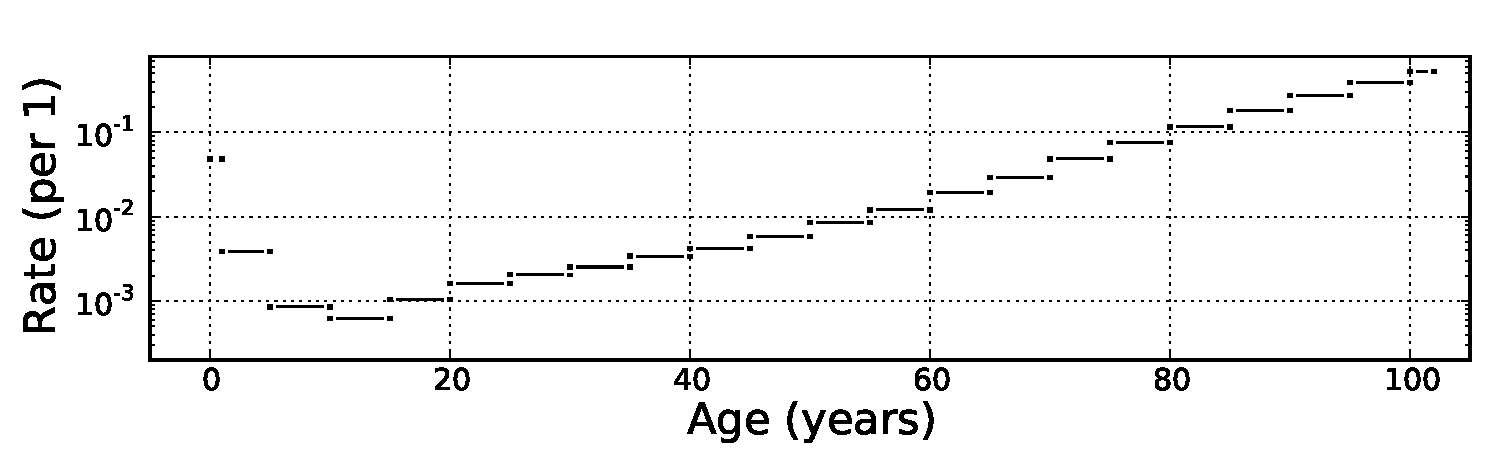
\includegraphics[width=\textwidth]{ssas-mx_female_1990.pdf}
\caption{All-cause mortality for females in the sub-Saharan Africa,
  Southern region in 1990 as a function of age shows the range of
  variation in age-specific rates.  $m_{\all}$ is as low as 6 per
  10,000 PY at age 10, but rises above 5,000 per 10,000 PY at age 100.}
\label{ssas-mx_female_1990}
\end{center}
\end{figure}

The approach that I have taken for modeling age-specific hazards draws
on the mathematical theory of spline interpolation, and the
statistical theory of penalized spline regression.  It is developed in
full detail in this chapter.


\section{Definition of splines models}

For my purposes, a spline model can be any piecewise polynomial
function.  Often I will require this function to be continuous, but
not always.  This is a departure from the conventions of statistical
spline modeling, which focuses on continuous and continuously
differentiable splines.\cite{hastie_elements_2009,wahba_spline_1990}

I represent a spline model for an age-specific hazard $h(a)$ by a set
of knots $a_1,\dots,a_{K}$, and a set piecewise polynomial basis
functions $\{p_1,\ldots,p_{K'}\}$.  Each knot has a corresponding
basis function, and for higher order splines, there may be additional
basis functions as well, so $K \leq K'$.  The model then has $K'$
parameters, $\gamma_1,\ldots,\gamma_{K'}$, and takes the form
\[
h(a) = \sum_{k=1}^{K'} \gamma_k p_k(a).
\]

The mathematical definition of the model is straight-forward, but the
detail of selecting the piecewise polynomials remains to be developed.
This is where the spirit of spline modeling lies. The knots $a_1,
\dots, a_{K}$ partition the age range into intervals. If I make each
piecewise polynomial $p_k(a)$ equal to $1$ on its interval (i.e., when
$a_k \leq a < a_{k+1}$) and zero otherwise, this yields a piecewise
constant spline model.  This is an important specialization, the
simplest of my spline models.  Using the notation $\1[a_k \leq a <
  a_{k+1}]$ to denote the function 
\[f(a)
= \begin{cases}1,&\quad\text{if }a_k \leq a <
  a_{k+1};\\0,&\quad\text{otherwise;}\end{cases}
\]
 and the convention
that $a_{K+1} = \infty$, I can write out the piecewise constant spline
model as
\[
h(a) = \sum_{k=1}^K \gamma_k \1[a_k \leq a < a_{k+1}].
\]

By taking the piecewise polynomial corresponding to each knot as zero
before its knot and a linearly increasing function after, the model
specializes to a piecewise linear spline model, a continuous
function that has a constant derivative at all non-knots.  By adding
an additional basis function that is not associated with a knot, this
piecewise linear spline model becomes a flexible approximation for any
nonlinear function, and is the main form I have used in representing
age-specific hazards in the work to come.  I can write out the
piecewise constant specialization of the spline model as
\[
h(a) = \gamma_0 + \sum_{k=1}^K \gamma_k a \1[a \geq a_k].
\]

I find that in applications of this model it is useful to represent
the piecewise linear spline in an alternative basis, where the model
parameter $\gamma_k$ represents the values of $h(a_k)$ instead of the
change in the slope at this point.  This yields a more complicated set
of basis functions, but it is not necessary to write out the basis
functions explicitly.


Figure~\ref{splines_fig} shows the results of fitting spline models
for age-specific hazards to simulated data to minimize the sum of the
square differences between the predicted and observed values.  When
the piecewise constant model is fit, it produces an age-specific
hazard function consisting of series of horizontal (constant) lines
in each of the intervals between knots.  Interval $k$ interval has
$\gamma_k$ equal to the mean value of the simulated data between knots
$a_k$ and $a_{k+1}$, which is quite a sensible choice.

A more favorable and flexible fit to the data is achieved by the
piecewise linear spline model, which produces a continuous function
of age as its prediction. In many cases, a piecewise linear fit of
this type is sufficient to capture the nonlinearity in the data, and
this will be the typical model for epidemiological rates in the second
half of this book.  It is possible to go further along this path of
smoothing, however, and splines that have continuous derivatives and
even continuous second derivatives are popular alternatives, achievable
by simply choosing different piecewise polynomials for the basis
functions.


\begin{figure}[h]
\begin{center}
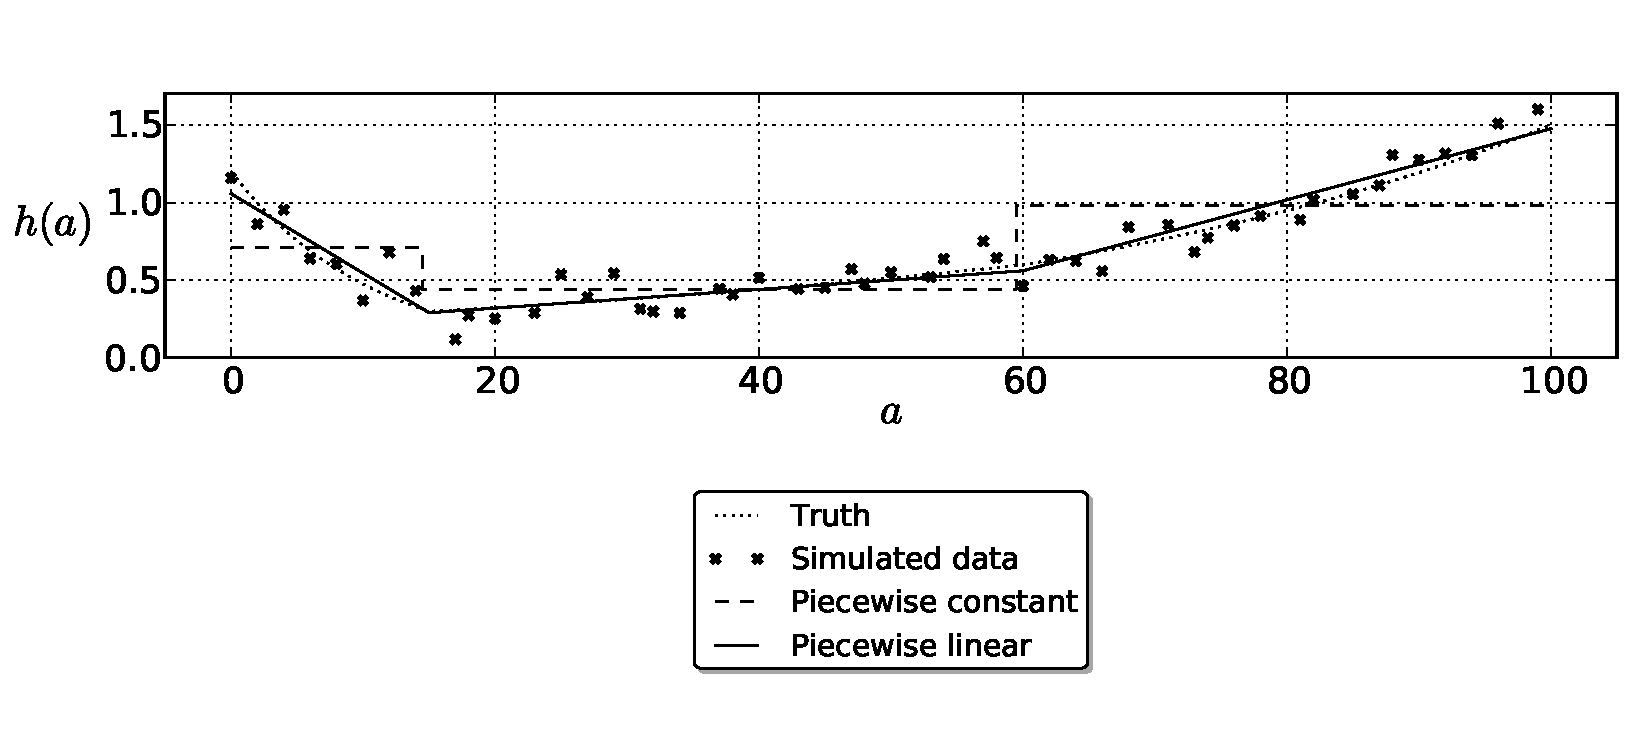
\includegraphics[width=\textwidth]{splines-fig.pdf}
\caption{Spline interpolation of simulated data. The true age-specific
  rate is piecewise log-linear, so none of the splines can represent
  it perfectly. The true age-specific rate and the models all have
  knot set $\{0, 15, 60, 100\}$.}
\label{splines_fig}
\end{center}
\end{figure}


\section{Choosing knots}

To this point, I have taken as given the number and location of the
knots in the spline model. However, selecting the number and location
of the knots is an important task, and, when working with sparse and
noisy data, this can influence the model results
substantially.

When data is abundant and age patterns are clear, models will not be
very sensitive to the choice of knots.  When data is not abundant, or
when the age patterns are not clear from the data, however, the knots
selection is an important part of the modeling process.  In this
setting, knot locations should be chosen a priori, based on expert
knowledge about the disease being modeling. For example, in a recent
study looking at global trends in mean systolic blood pressure as a
function of age, the modelers chose to use a cubic regression spline
with knots located at ages 30 and 60.\cite{danaei_national_2011} These
choices reflect the expectation, based on literature and prior
knowledge, that the behavior of mean systolic blood pressure as a
function of age would be distinct in these intervals due to low blood
pressure in young adults, and survivor effects in elderly populations.

Although this approach of using expert knowledge to inform the number
of knots and knot locations is practical and allows for users to
determine critical features of the model, it is certainly not the only
approach. Much literature is devoted to the choice of knot locations
and the number of knots.
An important direction for future work is to remove the reliance on
expert knowledge to inform knot selection.  This could proceed
through model selection or model averaging of models with a variety of
knot locations \cite{raftery_bayesian_1997}, through
techniques developed in the adaptive regression spline literature
\cite{friedman_multivariate_1991}, or by leaving spline models altogether and using Gaussian
processes or some similar nonparametric model for the age pattern
\cite{rasmussen_gaussian_2006,diggle_model-based_2010}.

\section{Penalized spline models}
One approach to address the challenge of knot selection is to include
more knots in the model and then also include a penalty function to
discourage the model from using the additional knots when the data
does not call for them.  This penalized spline model can be formulated in a
Bayesian framework by introducing a prior which represents the belief that, in
the absence of evidence, the age pattern is not varying.
Mathematically, this takes the form of a penalty on the root mean
square of the derivative of the age-specific rate $h(a)$:
\[
\left(\int _{a=a_1} ^{a_K} \| h'(a) \|^2 \d w(a)\right)^{1/2} \sim N(0, \sigma^2).
\]
This introduces an additional model parameter, $\sigma$, which can be
viewed as a hyperprior, and controls the amount of smoothing that the
penalty creates.

For the piecewise linear penalized splines that will be used most
frequently in the second half of this book, the derivative of $h$ is
constant between knots, so, with equal weighting for smoothing at all
ages, the integral above simplifies to the following:
\begin{align*}
\int _{a=a_1} ^{a_K} \| h'(a) \|^2 \d a
& = \sum_{k=1} ^{K-1} \left(\frac{h(a_{k+1}) - h(a_k)}{a_{k+1}-a_k}\right)^2 \frac{a_{k+1}-a_k}{a_K - a_1}\\
&= \sum_{k=1} ^{K-1} \frac{\left(h(a_{k+1}) - h(a_k)\right)^2}{(a_{k+1}-a_k)(a_K - a_1)}.
\end{align*}
Figure~\ref{smoothing-splines} shows the effect of increasing the
smoothing parameter $\sigma$, when many more knots than necessary have been included in the model.

\begin{figure}[h]
\begin{center}
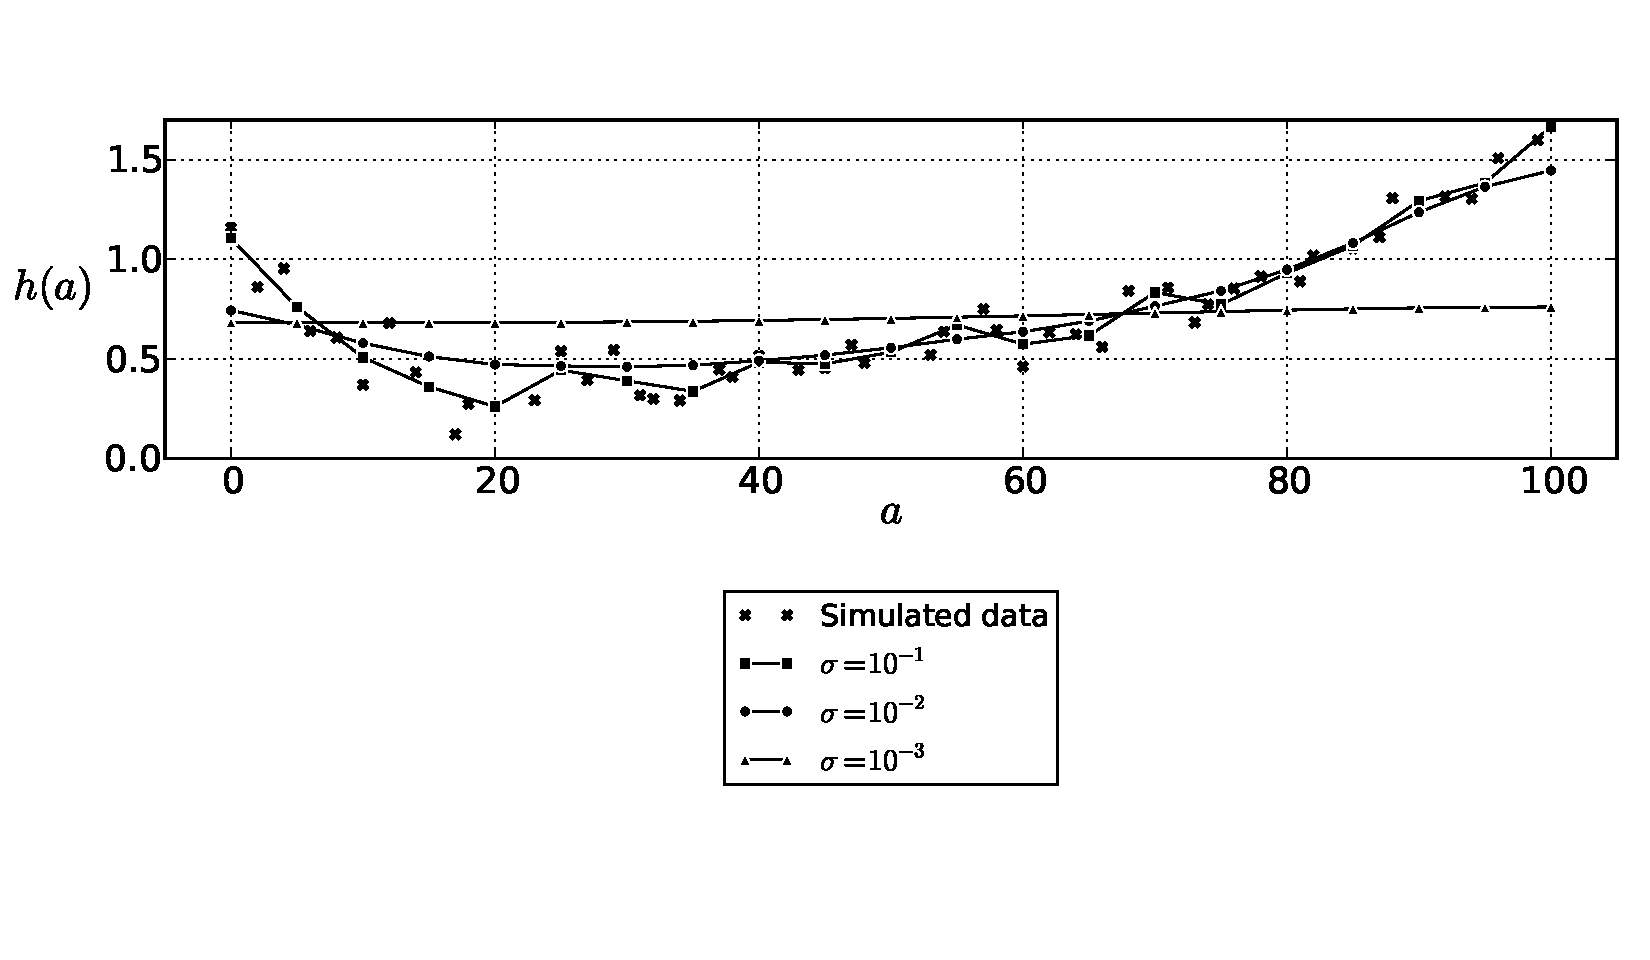
\includegraphics[width=\textwidth]{smoothing-splines.pdf}
\caption{Penalized splines with a carefully chosen smoothing parameter
  $\sigma$ provide a solution to the challenge of knot selection in
  spline modeling.  Without smoothing, including many knots leads to
  estimates that are overly uncertain and wiggly.  Smoothing, in the
  form of a quadratic penalty on the derivative of the age pattern,
  allows many knots to be included.  But too much smoothing, for
  example $\sigma=10^{-3}$ in this case, results in a model which does
  not reflect true patterns in the data.}
\label{smoothing-splines}
\end{center}
\end{figure}


\section{Augmenting the spline model}
There are a few ways to augment the spline model that are useful when
modeling age-specific rates. Since the epidemiological rates I have modeled
are always non-negative, I have parametrized the spline in
terms of the log of the knot values, so that $h(a)$ is a piecewise
linear spline model with knots $a_1,\ldots,a_K$, and
\[
h(a_k) = e^{\gamma_k}.
\]
In order to fit the model in a Bayesian framework, I have defaulted to
giving these $\gamma_i$'s ``weakly informative'' priors,
\[
\gamma_i \sim \Normal\left(0, 10^2\right).
\]
This has very little effect on the posterior distribution but makes
the prior ``proper'' and also helps with algorithm convergence in
some instances. In instances where relevant expert knowledge is
available, I can replace this with a more informative prior (this idea
is elaborated in the next section).

Finally, in order to deal with the order-of-magnitude differences of
age-specific rates, I have applied the smoothing penalty to the
logarithm of the rate, rather than the rate itself.  This creates an additional
complication, however, because the informative priors often say that
rates are zero for certain ages.  In order to avoid the ill effects of
smoothing when the rate contains values of $0$, I have
rounded up any $\gamma_i$ values that are below 10 times the mean
rate.  The approach is operationalized as a penalty term in the prior:
\[
\widetilde{\|h'\|} = \sqrt{\frac{\sum_{k=1}^{K-1}
\left(\max(\gamma_k, \gamma_{\min})
-
\max(\gamma_{k+1}, \gamma_{\min})\right)^2
}{(a_{k+1}-a_k)(a_K-a_1)}} \sim \Normal(0, \sigma^2),
\]
where $\gamma_{\min} = \log\left(\bigg(\sum_{i=0}^K e^{\gamma_i}/10\bigg)
/ K\right)$.


Taken all together then, the model for an age-specific hazard function
that will be used in this book is then:
\begin{align*}
h(a) &= \sum_{k=1}^{K-1} \1[a_k \leq a < a_{k+1}]
\left( \frac{a-a_k}    {a_{k+1}-a_k} e^{\gamma_k}
     + \frac{a_{k+1}-a}{a_{k+1}-a_k} e^{\gamma_{k+1}}\right),\\
\gamma_k &\sim \Normal\left(0, 10^2\right),\\
\widetilde{\|h'\|} &\sim \Normal(0, \sigma^2).\\
\end{align*}
The value of $\sigma$ is a model parameter that will receive an very
informative hyper-prior, for example ``slightly smooth'' is
represented by $\sigma=.1$.




\chapter{Expert priors on age patterns}
\label{theory-expert_priors}
\chapterprecis{Abraham D. Flaxman}

When dealing with sparse and noisy data, it is sometimes necessary to
include additional expert knowledge on the age pattern of
epidemiological rates.  For example, data sparsity can take the form
of a lack of information about age-specific hazards of disease in children.  In
diseases which are rare or nonexistent in children, the fact that incidence is
effectively zero before a certain age is known by disease experts but
not represented in the data collected by systematic review.

A benefit of the Bayesian methods that will be used to fit these
models is the conceptual and practical simplicity of adding additional
information to the age-pattern model.  This is implemented by choosing
a more informative prior distribution.  For example, if the
epidemiology of a disease is such that the incidence level must be
zero before age $a_k$, this can be incorporated by replacing the
weakly informative prior by the conditional probability density with
this constraint included.

There are three classes of additional information that will come up
frequently in the applications later in this book: level bound priors,
level value priors, and monotonicity priors. This section describes
how each can be implemented as an informative prior on the age pattern
model.


\section{Priors on level}

Informative priors on the level of the age pattern seem simple at
first but may have unintended effects.  A prior on the level value for
certain ages says precisely that the age pattern should have that
value for those ages.  For example, Figure~\ref{level-value-priors}
shows the effects of adding a prior where the age-specific hazard function takes values extremely
close to 0.1, 0.5, or 1.0 from age 0 to 15.


\begin{figure}[h]
\begin{center}
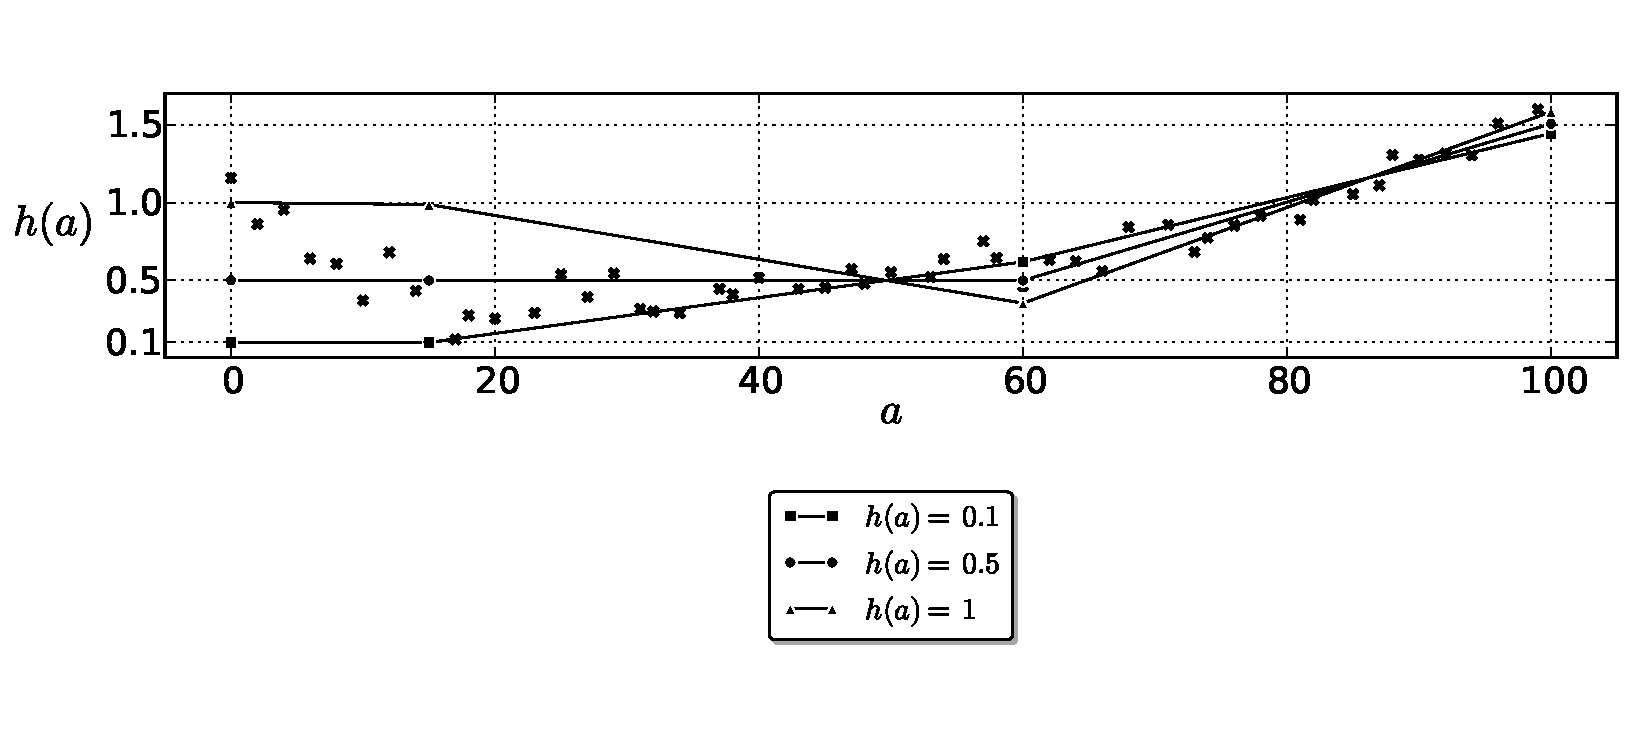
\includegraphics[width=\textwidth]{level_value-smoothing-splines.pdf}
\caption{An informative prior on the level of $h(a)$ for interval $0 \leq a <
  15$ changes the estimated rate dramatically for $a$ between $20$ and
  $60$ and even leads to different estimates for $a = 100$.  The more
  data available, the more knots in the model, and the lesser the
  smoothing penalty, the less this level value assumption will affect
  the estimates for ages outside of the interval, however.  }
\label{level-value-priors}
\end{center}
\end{figure}



These priors are implemented as ``hard-soft constraints''.  For a
value $v$ on age range $(a_0,a_1)$, the value of the spline model is
replaced with the level value for the age range (which I call a hard
constraint) and the prior density on the spline is augmented with a
penalty term for the offset-log difference between the level value of
the unconstrained spline and $v$ (which I call a soft constraint). The
offset-log difference penalty has the form:
\[
\log\left(h(a)+\e)\right) \sim
 \Normal\left(\log\left(v + \e\right), \sigma^2\right),
\]
where $h(a)$ is the age-specific hazard function, $\e = 10^{-6}$ is the
offset to avoid taking the log of zero, and $\sigma = 0.01$ is the
magnitude of the penalty.  In Bayesian terms, this encodes the belief
that the spline is expected to be within 1\% of the expert level
value, provided the level value is not too close to zero.

A similar sort of expert knowledge on the plausible bounds on
level is also useful, both in modeling noisy data and in increasing
the numerical stability of estimation algorithms. Again, however, the
implications of such a prior can be unexpected.
Figure~\ref{level-bounds-priors} shows the effects of three different
upper bounds on the spline estimation from the same dataset as the
previous figure.

\begin{figure}[h]
\begin{center}
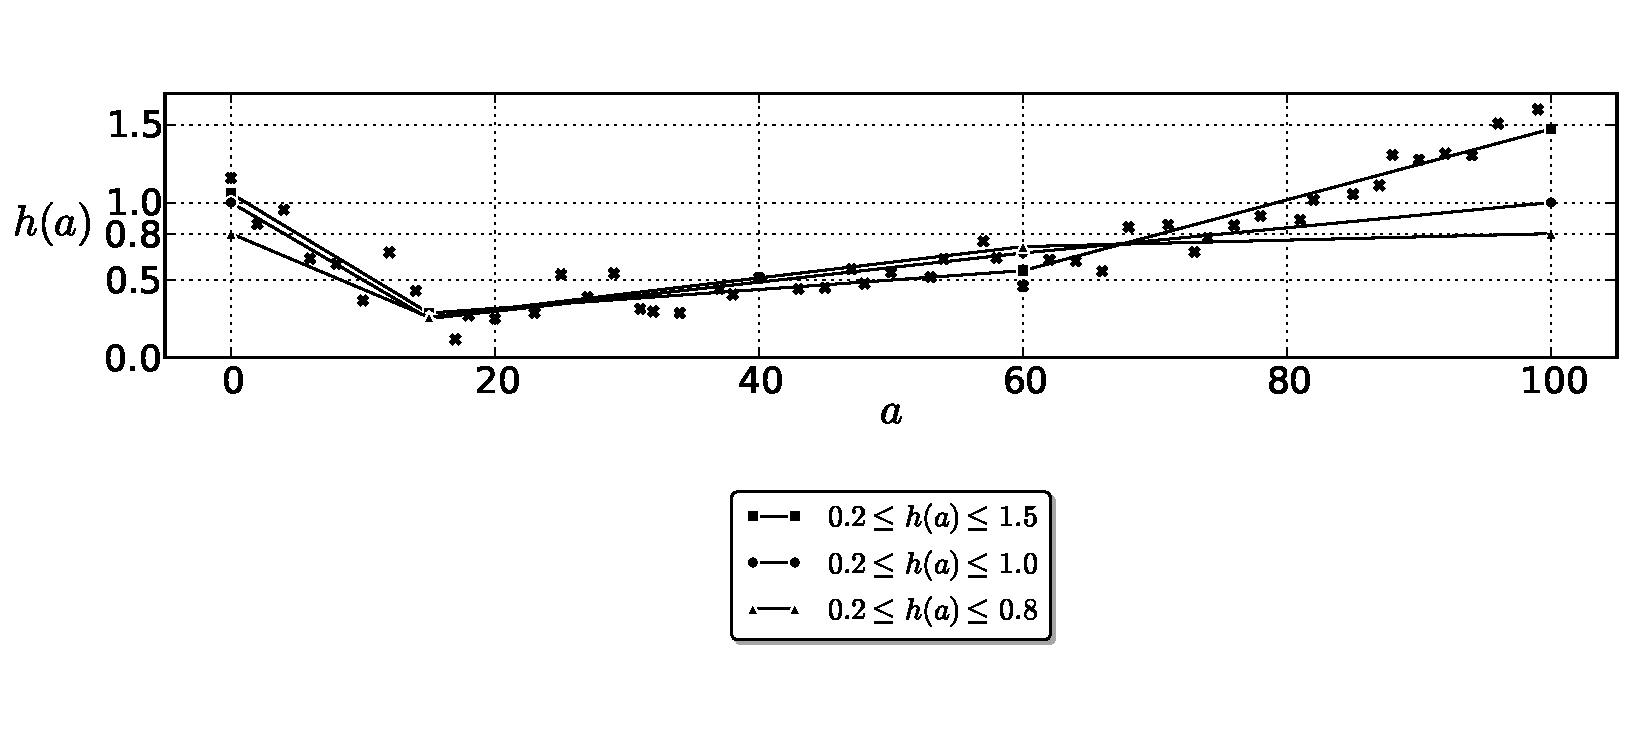
\includegraphics[width=\textwidth]{level_bound-smoothing-splines.pdf}
\caption{An informative prior on the upper and
lower bounds of age-specific hazard function $h(a)$ changes the estimated hazard function dramatically for
ages where the data are outside the bounds. For ages where the data are
inside the bounds, the estimates are also affected, but to a lesser
degree.}
\label{level-bounds-priors}
\end{center}
\end{figure}



Like the level value prior, this prior is also implemented as a
hard-soft constraint.  If the level bounds are $\ell_0 \leq h(a)
\leq \ell_1$, there is a hard constraint, that replaces the spline with a
clipped version, $h^c(a) = \clip(h(a), \ell_0, \ell_1)$, and a
also soft constraint that ensures that the original spline is close to the clipped
spline in offset-log-transformed space.

\section{Priors on monotonicity}

One common expert prior on age patterns is a strong belief that the
function is increasing or decreasing over a certain age
range. Mathematically speaking, these are priors on the sign of the
derivative of the age pattern.  These priors can be implemented efficiently in
Bayesian Markov chain Monte Carlo (MCMC) computation by conditioning on the differences of the
age-specific hazard function $h(a)$, for example:
\[
h(a) \geq h(a+1) \text{ for } a : a_s < a < a_e.
\]

The results of such a prior are shown in
Figure~\ref{monotone-age-pattern}.


\begin{figure}[h]
\begin{center}
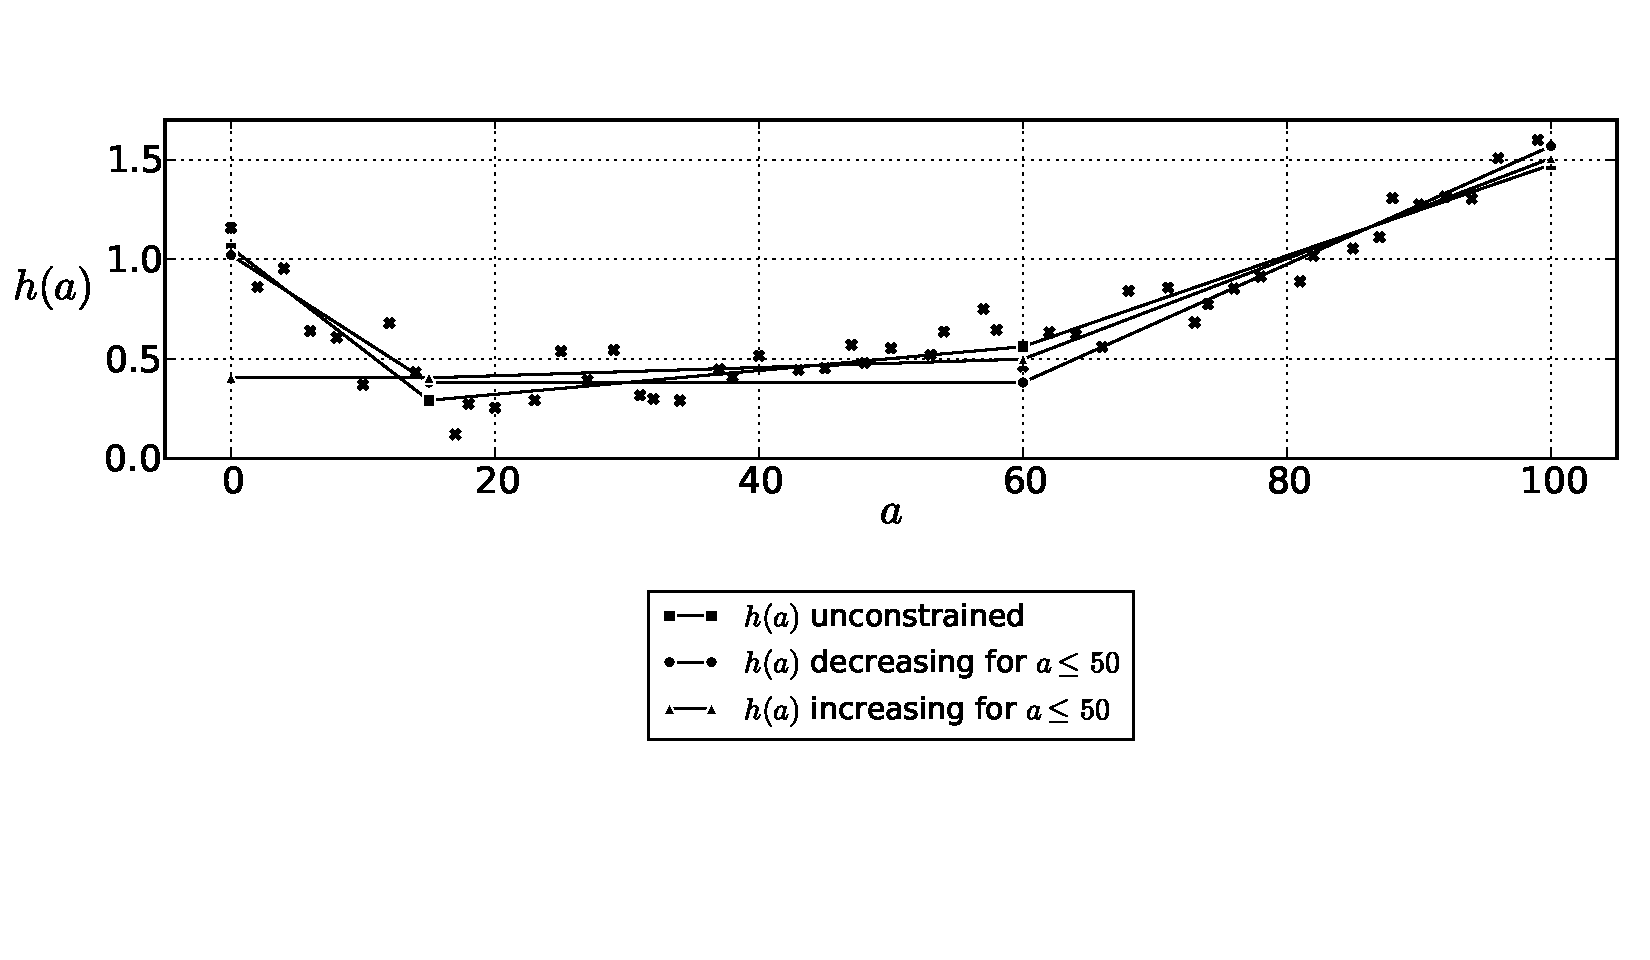
\includegraphics[width=\textwidth]{monotone-smoothing-splines.pdf}
\caption{The expert belief that the age pattern is increasing or is
  decreasing across an age range can also be implemented as a Bayesian
  prior.  When the prior is contrary to the data the estimate will be
  as close to the data as possible while respecting the prior.  For
  example, the age-specific hazard function marked with triangles is the result
  of a prior belief that the age pattern is increasing from age $0$ to
  $50$ when confronted with data shown as x-shaped markers that
  clearly do decrease over this age range.}
\label{monotone-age-pattern}
\end{center}
\end{figure}


For computational efficiency, the increasing and decreasing
constraints are implemented as soft constraints.  For a constraint
that the function is decreasing between $a_s$ and $a_e$, I include the penalty
\[
\operatorname{clip}(\log h(a+1) - \log h(a), 0, 1) \sim \Normal(0, \epsilon^2),
\]
for a small value of $\epsilon$, like $\epsilon = 10^{-6}$.  This has
a fully Bayesian interpretation, encoding a belief that a decreasing age pattern is expected
and an increase of more than approximately .0003\% is very surprising.


An area for future work comes from another common expert belief that
the age pattern is unimodal.  This is conceptually clear, but
computationally it has proven more difficult to realize than
monotonicity.  While the monotonicity constraint maintains
log-concavity of the posterior distribution (if it was log-concave to
start with), a straightforward implementation of a unimodality
constraint will result in nonlog-concave posterior distribution, even
if everything else is well behaved.  This suggests that the difficulty
in fitting such models in inherent in the local step method of the
MCMC algorithms I have been using.  Perhaps an alternative approach
such as the population Monte Carlo algorithm would be more successful.
Alternatively, there are some approximations of the unimodality
constraint that may be easier to optimize over \cite{papp_shape_2012}.

\section{Priors are not just for splines}
All three of the expert priors developed in this section are
applicable to any age-specific function derived from the compartmental
model in Chapter~\ref{sys-dynamics}. Most importantly, the
age-specific prevalence $p(a) = C(a)/(S(a)+C(a))$ can be augmented with expert
priors on level values (e.g., birth prevalence is zero), level bounds
(e.g., no population has prevalence above 10\%), and monotonicity
constraints (e.g., prevalence in increasing as a function of
age). Relative mortality risk $\frac{h_m(a)+h_f(a)}{h_m(a)}$ is another derived quantity that
experts often have strong priors about.

However, this sort of modeling requires care. The system dynamics
model enforces a precise consistency between the different
epidemiological rates, and making strong assumptions about one will
have implications for others.  Sometimes these implications are
counterintuitive.

As a practical matter, I recommend modeling begin with as few
assumptions as possible and gradually add in expert priors. The
benefit of this is threefold.  First, fitting the model without all of
the available expert knowledge allows the data to speak.  If the estimates
confirm the expert belief that is reassuring, and if it shows the
opposite, that is interesting. Second, the MCMC algorithm has a
pitfall: \emph{nonconvergence}. A quick way into this pit is
introducing inconsistent expert priors, for example, decreasing
prevalence and prevalence of zero at age $0$. By adding in expert
priors one at a time, the inconsistency that caused nonconvergence
will be more easily identified. Third, as with any model that produces
estimates from sparse and noisy data, it is essential to conduct a
sensitivity analysis to understand how influential modeling
assumptions are on the results.  The gradual addition of expert priors
will provide a starting point for this sensitivity analysis, showing
which expert priors are essential to obtaining reasonable results and
which are not as critical.

\section{Empirical priors on age patterns}
Another type of level prior worthy of separate exposition is that used
to implement the empirical Bayes approach that permits decomposing the
global estimation computation into region subcomputations that can be
run in parallel.  If estimates of the mean and standard deviation of
an age pattern are known for each age from a prior computation, this
information can be included into the age-specific hazard through a
penalty of the form
\[
h(a) \sim \Normal\left(\boldmu_{\text{prior}}(a),
\boldsigma_{\text{prior}}^2(a)\right).
\]

Since the model must cope with the order-of-magnitude differences of age-specific rates, it can be more robust to use an empirical prior relating the offset-log transformed rates:
\[
\log(h(a)+\epsilon) \sim \Normal\left(\log(\boldmu_{\text{prior}}(a)+\epsilon),
\left(\frac{\boldsigma_{\text{prior}}+\epsilon}{\boldmu_{\text{prior}}+\epsilon}\right)^2\right).
\]
